% !TeX spellcheck = it_IT
\newpage

\section{Algoritmi}
\subsection{Divide et impera}
È una tecnica di risoluzione di problemi che consiste in tre passi:
\begin{itemize}
	\item \textbf{Dividere} il problema in 2 o più sotto problemi identici ma di dimensione ridotta rispetto a quello originale
	\item \textbf{Risolvere} i sotto problemi \emph{ricorsivamente}
	\item \textbf{Combinare} le soluzioni dei sotto problemi per ottenere la soluzione del problema iniziale
\end{itemize}
\subsection{Ordinamento}
\begin{definition}[Algoritmo stabile]
	Un algoritmo di ordinamento si dice stabile quando preserva l'ordine iniziale tra due elementi con la stessa chiave.
\end{definition}
\subsubsection{Merge sort}
L'idea è di usare la tecnica precedentemente descritta del \textbf{Divide et Impera} e di spezzare l'array in due sotto-array di uguale dimensione, ordinarli e poi fonderli in uno unico. \\
La fusione verrà fatta confrontando i primi due elementi di ogni sotto-array, copiando il più piccolo nell'array finale, e proseguendo con il confronto del più grande con il successivo.
\begin{figure}[h]
	\begin{subfigure}{.5\textwidth}
		\centering
		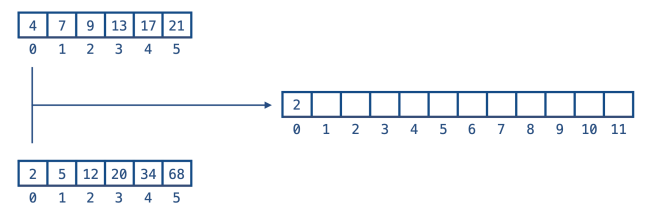
\includegraphics[width=8cm]{images/mergesort_1.png}
	\end{subfigure}
	\begin{subfigure}{.5\textwidth}
		\centering
		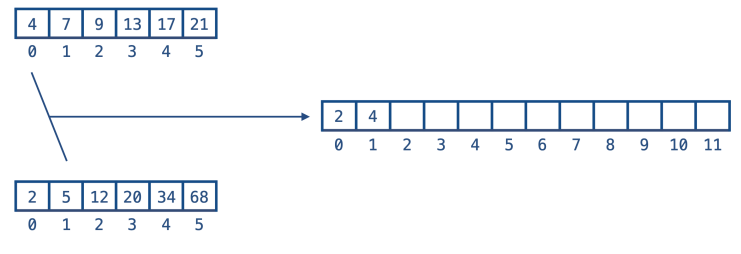
\includegraphics[width=8cm]{images/mergesort_2.png}
	\end{subfigure}
\end{figure}
\begin{figure}[h]
	\begin{subfigure}{.5\textwidth}
		\centering
		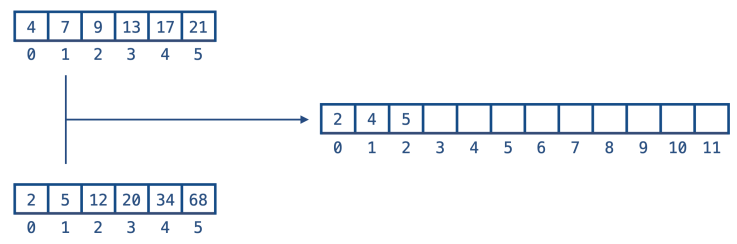
\includegraphics[width=8cm]{images/mergesort_3.png}
	\end{subfigure}
	\begin{subfigure}{.5\textwidth}
		\centering
		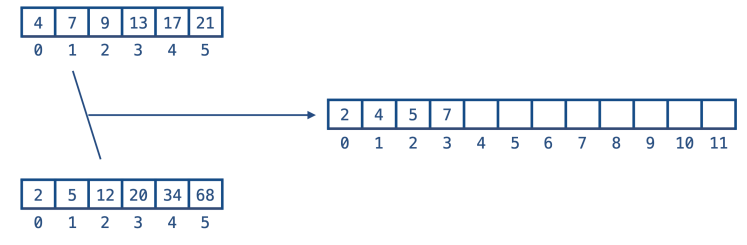
\includegraphics[width=8cm]{images/mergesort_4.png}
	\end{subfigure}
\end{figure}

\noindent Esempio di implementazione:

\begin{lstlisting}[language=C, caption=Algoritmo merge sort, mathescape=true]
	void merge_sort(int a[], size_t dim, char order) {
		sort(a, 0, dim-1, order);
	}

	void sort(int a[], size_t inizio, size_t fine, char order) {
		if ((fine - inizio) >= 1) {
			// Passo ricorsivo
			size_t centro1 = (inizio + fine)/2;
			zie_t centro2 = centro1 + 1;
			
			sort(a, inizio, centro1, order);
			sort(a, centro2, fine, order);
			
			merge(a, inizio, centro1, centro2, fine, order);
		}
		// Il caso base non serve, un array di un elemento e' ordinato
	}
	
	void merge(int a[], size_t sin, size_t centro1, size_t centro2, size_t dx, char order) {
		size_t sin i = sin;
		size_t dx_i = centro2;
		size_t fondi i = 0;
		int temp_a[dx - sin + 1];
		
		while (sin_i <= centro1 && dx_i <= dx) {
			switch (order) {
				case 'I':				
					if (a[sin_i] <= a[dx_i]) {
						temp_a[fondi_i++] = a[sin_i++];
					} else {
						temp_a[fondi_i++] = a[dx_i++];
					}
					break;
				default:
					if (a[sin_i] <= a[dx_i]) {
						temp_a[fondi_i++] = a[dx_i++];
					} else {
						temp_a[fondi_i++] = a[sin_i++];
					}
					break;
			}
		}
		
		// Se esaurisco il sotto-array sinistro
		if (sin_i == centro2) {
			while (dx_i <= dx) {
				temp_a[fondi_i++] = a[dx_i++];
			}
		} else {
			// Se esaurisco quello destro
			while (sin_i <= centro1) {
				temp_a[fondi_i++] = a[sin_i++];
			}
		}
	
		// Copio l'array temporaneo in quello originale
		for (size_t i = sin; i <= dx; i++) {
			a[i] = temp_a[i-sin];	
		}
	}
\end{lstlisting}

\subsubsection{Insertion sort}
\textbf{Proprietà}: al termine del passo j-esimo dell'algoritmo l'elemento j-esimo viene in inserito al posto giusto e i primi $j+1$ elementi sono ordinati.
\begin{lstlisting}[language=Javascript, caption=Algoritmo insertion sort, mathescape=true]
	insertionSort(A) =
	var j:Int = 0;
	var i:Int = 0;		$\Theta(1)$
	var k:int = 0;
	for (j=1; j<n; j++) {		$n-1$ volte
		k = A[j];
		i = j-1;		$\Theta(1)$ $n-1$ volte
		while(i >= 0 && A[i]>k) {
			A[i+1] = A[i];			$\Theta(1)$ $\sum\limits_{j=1}^{n-1} (t_j-1)$ volte
			i=i-1;
		}
		A[i+1] = k;		$\Theta(1)$ $n-1$ volte
	}
\end{lstlisting}

\begin{table}[h]
	\centering
	\begin{tabular}{ |c|c|c|c|c|c| }
		\hline
		0 & 1 & 2 & 3 & 4 & 5 \\
		\hline
		5 & 2 & 4 & 6 & 1 & 3 \\
		\hline 
		5 & 2 & 4 & 6 & 1 & 3 \\
		\hline 
		5 & 5 & 4 & 6 & 1 & 3 \\
		\hline 
		2 & 5 & 4 & 6 & 1 & 3 \\
		\hline 
		2 & 5 & 4 & 6 & 1 & 3 \\
		\hline 
		2 & 5 & 5 & 6 & 1 & 3 \\
		\hline 
		2 & 4 & 5 & 6 & 1 & 3 \\
		\hline 
		2 & 4 & 5 & 6 & 1 & 3 \\
		\hline 
		2 & 4 & 5 & 6 & 1 & 3 \\
		\hline 
	\end{tabular}
	\begin{tabular} { |c|c|c|c|}
		\hline
		j & i & k & while \\
		\hline
		0 & 0 & 0 & no \\
		\hline
		1 & 0 & 2 & si \\
		\hline
		1 & -1 & 2 & no \\
		\hline
		1 & -1 & 2 & no \\
		\hline
		2 & 1 & 4 & si \\
		\hline
		2 & 0 & 4 & no \\
		\hline
		2 & 0 & 4 & no \\
		\hline
		3 & 2 & 6 & no \\
		\hline
		3 & 2 & 6 & no \\
		\hline
	\end{tabular}
	\caption{Esempio di esecuzione}
\end{table}
\textbf{Complessità}:
\begin{align*}
	\sum\limits_{j=1}^{n-1} t_j
\end{align*}
\begin{itemize}
	\item Caso pessimo: l'array è ordinato decrescente e quindi ogni volta devo scalare l'elemento fino alla prima posizione. Abbiamo che $t_j = j$ e $\sum\limits_{j=1}^{n-1} j = \frac{n(n-1)}{2}$, quindi $O(n^2)$
	\item Caso migliore: l'array è ordinato crescente e quindi per ogni iterazione non entro nel while perché la condizione è falsa. Abbiamo $t_j = 1$ e $\sum\limits_{j=1}^{n-1} j = n-1$, quindi $O(n)$
	\item Caso medio: come il caso pessimo $O(n^2)$
\end{itemize}
\textbf{Correttezza}:
\begin{itemize}
	\item dimostro l'\textbf{invariante di ciclo} per assicurarmi che la mia proprietà venga mantenuta durante tutta l'esecuzione. Lo faccio tramite \emph{induzione}:
	\begin{itemize}
		\item Caso base: per $j=1$
		\item Hp induttiva: per $j=n'$
		\item Passo induttivo: dimostro che vale anche per $j=n'+1$
	\end{itemize}
	\item verifico la \textbf{terminazione}: il \emph{for} è eseguito esattamente $n-1$ volte e il \emph{while} al più $j-1$ volte, quindi tutte le iterazioni sono finite e l'algoritmo termina.
\end{itemize}
\textbf{Memoria impiegata}: ordina in loco quindi non usa memoria aggiuntiva.

\subsubsection{Selection sort}
\textbf{Proprietà}: al termine del passo j-esimo dell'algoritmo i primi $j+1$ elementi di A sono ordinati e contengono i $j+1$ elementi più piccoli di A.
%TODO Calcolo della complessità non corretto
\begin{lstlisting}[language=Javascript, caption=Algoritmo selection sort, mathescape=true]
	insertionSort(A) =
	var j:Int = 0;
	var i:Int = 0;		$\Theta(1)$
	var min:int = 0;
	for (i=0; i<n-1; i++) {		$n-1$ volte
		min = i;		$\Theta(1)$ $n-1$ volte
		for(j=i+1; j<n; j++) {
			if A[j] < A[min] {min = j};			$\Theta(1)$ $\sum\limits_{j=1}^{n-1} (t_j-1)$ volte
		}
		swap(A[i],A[min]);		$\Theta(1)$ $n-1$ volte
	}
\end{lstlisting}
\begin{table}[h]
	\centering
	\begin{tabular}{ |c|c|c|c|c|c| }
		\hline
		0 & 1 & 2 & 3 & 4 & 5 \\
		\hline
		5 & 2 & 4 & 6 & 1 & 3 \\
		\hline 
		1 & 2 & 4 & 6 & 5 & 3 \\
		\hline 
		1 & 2 & 4 & 6 & 5 & 3 \\
		\hline 
		1 & 2 & 3 & 6 & 5 & 4 \\
		\hline 
		1 & 2 & 3 & 4 & 5 & 6 \\
		\hline 
		1 & 2 & 3 & 4 & 5 & 6 \\
		\hline
	\end{tabular}
	\begin{tabular} { |c|c|c|}
		\hline
		j & i & min \\
		\hline
		0 & 0 & 0 \\
		\hline
		1 & 0 & 4 \\
		\hline
		2 & 1 & 1 \\
		\hline
		3 & 2 & 5 \\
		\hline
		4 & 3 & 3 \\
		\hline
		5 & 4 & 4 \\
		\hline
	\end{tabular}
	\caption{Esempio di esecuzione}
\end{table}
\textbf{Complessità}
%TODO Inserisci il calcolo della complessità
\begin{align*}
	\sum\limits_{j=1}^{n-1} j = \frac{n(n-1)}{2} \in O(n^2)
\end{align*}
\begin{itemize}
	\item Caso pessimo: $O(n^2)$
	\item Caso migliore: $O(n^2)$
	\item Caso medio: $O(n^2)$
\end{itemize}
\textbf{Correttezza}:
\begin{itemize}
	\item dimostro l'\textbf{invariante di ciclo} per assicurarmi che la mia proprietà venga mantenuta durante tutta l'esecuzione. Sempre tramite induzione.
	\item verifico la \textbf{terminazione} in maniera analoga all'insertion sort.
\end{itemize}
\textbf{Memoria impiegata}: ordina in loco quindi non usa memoria aggiuntiva.

\subsubsection{Bubble sort}
Questo algoritmo scorre l'array e, a coppie, ordina gli elementi facendo più passate. Il nome \emph{bubble} deriva dal fatto che ad ogni passata i numeri più grandi (o piccoli) si spostano verso la fine dell'array come le bolle d'aria salgono a galla.
\begin{lstlisting}[language=C, caption=Algoritmo bubble sort, mathescape=true]
	void bubble_sort (int a[], size_t dim, char order) {
		int temp;
		for (unsigned int passate = 0; passate < dim; passate++) {
			for (size_t i=0; i < (dim - 1); i++) {
				switch (order) {
					case 'I':
						if (a[i] > a[i+1]) {
							temp = a[i];
							a[i] = a[i+1];
							a[i+1] = temp;
						}
						break;
					default:
						if (a[i] < a[i+1]) {
							temp = a[i];
							a[i] = a[i+1];
							a[i+1] = temp;
							 break;
						}
				}
			}
		}
	}
\end{lstlisting}
\textbf{Complessità}\\
Il primo \emph{for} esegue $n$ cicli e quello interno ne esegue $n-1$. Di conseguenza la complessità è $n\cdot (n-1)$, ovvero $\mathbf{n^2}$.
\subsection{Linear sort}
Gli algoritmi di ordinamento di questo tipo sfruttano il fatto che l'array da ordinare abbia determinate proprietà.
\begin{example}
	Dato un array $A$ di $n$ interi compresi tra $1$ e $k$:
	\begin{align*}
		\forall 0 < j \leq n . A[j] \in [1, \ldots, k]
	\end{align*}
	\begin{lstlisting}[language=Javascript, caption=Algoritmo linear sort, mathescape=true]
		linearSort(A:[Int], B:[Int], k:Int) -> Void {
			// Inizializzo un array che tiene conto dei numeri da 1 a k
			for (var i:Int = 1; i<=k; i++) C[i] = 0;	$\Theta(k)$
			
			var j:Int = 1;
			// Conto quante volte compare ogni numero nell'array originale
			for (j=1; j<=n; j++) C[A[j]] += 1;	$\Theta(n)$
				
			j=1;
			var z:Int = 1;
			// Dispongo ogni numero nell'array finale in ordine sapendo quante volte compare
			for (z=1; z <= k; z++) {	$\Theta(k)$
				for (var v:Int = 0; v < C[z]; v++) {	$\Theta(n)$
					B[j] = z;
					j++;	
				}	
			}	
		}
	\end{lstlisting}
	\textbf{Complessità}\\
	In questo caso la complessità è $\Theta(n + k)$ e si usa quando $k \in O(n)$.
\end{example}
\subsubsection{Radix sort}
Questo algoritmo funziona in maniera simile a come il cervello umano ordina gruppi di numeri: si ordinano (tramite un algoritmo di ordinamento \textbf{stabile} prima le cifre delle migliaia, poi quelle delle centinaia, quelle delle decine ed infine le unità. Notiamo però che il risultato NON è corretto.
\begin{table}[h]
	\centering
	\begin{tabular}{ccccc}
		\textbf{1}094 & \textbf{9}86 & 10\textbf{9}4 & 12\textbf{5} & 1120 \\
		986 & \textbf{2}34 & 1\textbf{2}5 & 112\textbf{0} & 234 \\
		234 & \textbf{1}25 & 11\textbf{2}0 & 23\textbf{4} & 1094 \\
		125 & 1\textbf{0}94 & 2\textbf{3}4 & 98\textbf{6} & 125 \\
		\textbf{1}120 & 1\textbf{1}20 & 9\textbf{8}6 & 109\textbf{4} & 986
	\end{tabular}
\end{table}
\\
Per farlo funzionare dobbiamo ordinare le cifre partendo da quelle meno significative, quindi dalle unità.
\begin{table}[h]
	\centering
	\begin{tabular}{ccccc}
		109\textbf{4} & 11\textbf{2}0 & 1\textbf{1}20& \textbf{1}094 & 125 \\
		98\textbf{6} & 10\textbf{9}4 & \textbf{1}25 & \textbf{1}120 & 234 \\
		23\textbf{4} & 2\textbf{3}4 & \textbf{2}34 & 125 & 986 \\
		12\textbf{5} & 1\textbf{2}5 & \textbf{9}86 & 234 & 1094 \\
		112\textbf{0} & 9\textbf{8}6 & 1\textbf{0}94 & 986 & 1120
	\end{tabular}
\end{table}